\documentclass[xetex,aspectratio=43]{beamer}

\usepackage{res/lections}

\preamble

\title[Устройство и принципы проектирования ЦП]{Общее устройство центрального процессора~и принципы его проектирования}

\begin{document}

    \titleslide

    \tocslide

\section{Блоки процессора}

\begin{frame}{Арифметико-логическое устройство}
    \defn{Арифметико-логическое устройство}{блок процессора, выполняющий арифметические и логические операции}
    \begin{itemize}
        \item В простейшем случае --- просто логическая схема
        \item Может использоваться для прикладных (например, вычисления, заданные программистом) и служебных (например, адресная арифметика)
        \item Имеет несколько входов для операндов и выход, на который \emph{мультиплексируются} выходы сумматора, мультипликатора и т.д.
    \end{itemize}
\end{frame}

\begin{frame}{Регистровый файл}
    \defn{Регистровый файл}{блок процессора, включающий набор регистров; внутренняя память процессора}
    \begin{outline}[itemize]
        \tightlist
        \1 Арифметические регистры
            \2 Аккумулятор
            \2 Ещё несколько [десятков] регистров
        \1 Регистры состояний
            \2 Регистр флагов
        \1 Адресные регистры
            \2 Указатель вершины стека
            \2 Указатель на текущую инструкцию
            \2 Указатель на данные [часто несколько]
            \2 Вспомогательные (например, сегментные)
        \1 Служебные регистры
            \2 Хранение промежуточных значений, реализация протоколов (например, с ОЗУ) и т.д.
    \end{outline}
\end{frame}

\begin{frame}{Блок выборки инструкций (устройство чтения программы)}
    \defn{Блок выборки инструкций}{блок процессора, выполняющий чтение очередных инструкций из памяти}
    \begin{outline}[itemize]
        \1 Читает из ОЗУ машинный код
            \2 Выполняет первичную интерпретацию машинного кода
    \end{outline}
    Для CISC-процессоров со сложным машинным кодом это не так-то просто!

    \pause
    \alert{О том, что такое RISC и CISC, ещё немного позже.}
\end{frame}

\begin{frame}{Управляющее устройство}
    \defn{Управляющее устройство}{блок процессора, выдающий для исполнения машинных команд управляющие сигналы другим блокам}
    \begin{outline}[itemize]
        \1 В зависимости от команды, выдаёт управляющие сигналы другим блокам процессора
            \2 Сигналы преимущественно управляют мультиплексорами, т.е. задают \emph{маршруты передачи данных между блоками процессора}
        \1 Если команда выполняется за много тактов (а обычно так и есть), выдаёт не один сигнал, а \emph{последовательность сигналов} разным блокам
    \end{outline}
\end{frame}

\section{Одно-, многотактный процессоры}

\begin{frame}{Однотактная схема}
    \begin{figure}
        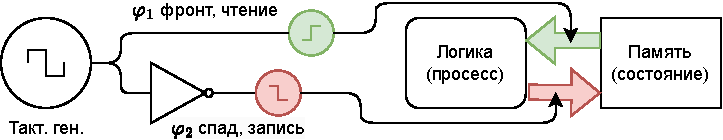
\includegraphics[width=\textwidth, page=1]{img/11.CPUS.drawio-crop.pdf}
    \end{figure}
    Вспоминаем:
    \begin{outline}[enumerate]
        \1 Синхронные и асинхронные вычисления, тактовый генератор, тактовые импульсы и тактовую сеть
        \1 Синхронизацию по фронту и спаду тактового импульса
        \1 Связку «master-slave»
        \1 Многофазные тактовые сигналы у старых процессоров
    \end{outline}
\end{frame}

\begin{frame}{Однотактный процессор}
    \begin{figure}
        \includegraphics[width=0.75\textwidth, page=2]{img/11.CPUS.drawio-crop.pdf}
    \end{figure}

    \begin{outline}[itemize]
        \1 В принципе, он даже может работать
            \2 Можно «нарисовать», например, несложный контроллер с такой архитектурой
        \1 Только гарвардский, т.к. нельзя одновременно обращаться и в одну память за кодом и данными
    \end{outline}
\end{frame}

\begin{frame}{Многотактный процессор (упрощённый пример для 3 тактов)}
    \vspace{-2mm}
    \begin{figure}
        \includegraphics[width=0.95\textwidth, page=3]{img/11.CPUS.drawio-crop.pdf}
    \end{figure}
    \vspace{-2mm}

    \begin{outline}[itemize]
        \1 Используются три фазы --- $\varphi_0, \varphi_1, \varphi_2$
            \2 Эти фазы может генерировать процессор внутри себя по сигналам обычного тактового генератора
        \1 Разные фазы выполняются разными блоками по очереди
            \2 $\frac{2}{3}$ времени блоки процессора простаивают!
    \end{outline}
\end{frame}

\section{Конвейеризация}

\subsection{Конвейеры в реальной жизни}

\begin{frame}{Конвейеризация «в жизни»}
\begin{block}{Предпосылки}
    Эли Уитни, 1798 (оружейное производство) — одновременное изготовление стандартизованных узлов мушкета разными рабочими, затем быстрая сборка готовых изделий
\end{block}

\begin{block}{Реальные конвейеры}
    \begin{outline}[itemize]
        \1 Генри Форд, 1913 и т.д. — сборка электрогенераторов, затем моторов и целых автомобилей
            \2 Разные этапы производства выполняются разными рабочими
            \2 Рабочие работают одновременно, каждый на своём этапе
        \1 Конвейер в системе образования
            \2 Школа: 1–11 классы — выпуск каждый год, но школьник учится 11 лет
            \2 Высшее образование: \emph{старая} поговорка: Матмех — не школа, за \emph{10 лет} не окончишь =)
        \1 Конвейер в менеджменте
            \2 Конвейерное исполнение заказов
    \end{outline}
\end{block}
\end{frame}

\begin{frame}{Недостатки конвейера}
    \begin{outline}[itemize]
        \1 Низкая гибкость — организованный и запущенный конвейер тяжело приспособить к изменяющейся ситуации
        \1 Снижение качества результата в угоду массовости
            \2 Пример: товар есть на складе в моём городе, но почему-то едет с другого конца страны
    \end{outline}
    \pause
    Выход: в менеджменте это преодолевается переходом от конвейера к организации бизнес-процессов — сложнее, но адаптивнее
\end{frame}

\subsection{Вычислительные конвейеры}

\begin{frame}{Что такое конвейер?..}
    \defn{Вычислительный конвейер (водопровод, pipeline)}{механизм распараллеливания выполнения машинных команд, позволяющий оптимально задействовать блоки процессора путём разбиения команд на стадии и распределения стадий по блокам}

    ~

    Конвейеры появились в 1950-х годах, термин «конвейер» (pipeline) ввёл конструктор советских ЭВМ С.А. Лебедев.

    ~

    Пусть все команды выполняются за $N$ тактов. Тогда, что даёт конвейеризация?

    \begin{outline}[itemize]
        \1 Скорость выполнения отдельных команд:
            \2 Каждая команда выполняется за $N$ тактов как с конвейером, так и без
            \2 В отношении одной команды на разных тактах задействованы разные блоки
        \1 Скорость выполнения программы:
            \2 На каждом такте завершается очередная команда
            \2 Конвейеризация ускоряет работу программы в $N$ раз, все блоки задействованы всё время
            \pause
            \2 Косвенная выгода: «сосредоточение» отдельных стадий в компактных блоках позволяет увеличить тактовую частоту
    \end{outline}

\end{frame}


\begin{frame}{Пример: Classic RISC Pipeline}
    \begin{figure}
        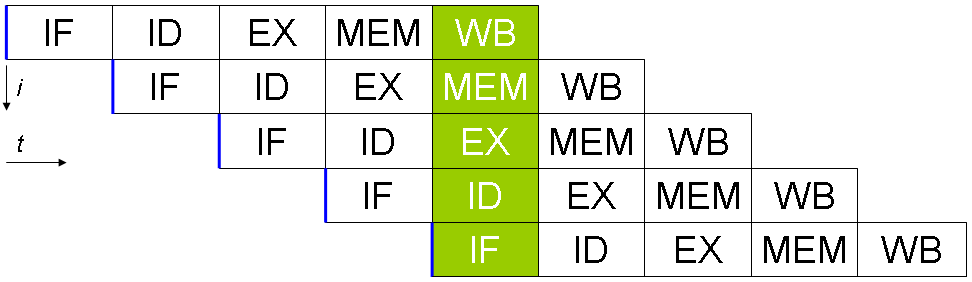
\includegraphics[width=0.7\textwidth]{img/11.classic-RISC-pipeline.png}
        \caption{Classic RISC Pipeline, Wikipedia}
    \end{figure}
    Применялся к популярным RISC-процессорам 1980-х: первым MIPS, Sun SPARC, Motorla 88000.
    Стадии:
    \begin{enumerate}
        \tightlist
        \item IF (instruction fetch) — получение инструкции
        \item ID (instruction decode) — декодирование инструкции
        \item EX (execute) — выполнение инструкции, если нужно — первый такт доступа к данным в ОЗУ
        \item MEM memory access) — второй такт доступа к данным в ОЗУ или бездействие
        \item WB (register write back) — запись в регистр
    \end{enumerate}
\end{frame}

\begin{frame}{Проблемы конвейеризации}
    \begin{outline}[enumerate]
        \renewcommand{\outlineii}{itemize}
        \1 Конфликты по данным между зависимыми машинными командами, например:
            \2 самая частая ситуация — следующей команде нужен результат предыдущей, но предыдущая ещё его не получила
            \2 следующая команда записывает данные до того, как их читает предыдущая
            \2 следующая команда записывает свои результаты раньше предыдущей из-за чего предыдущая потом может их перезаписать

        \1 Конфликты по ресурсам — когда двум командам одновременно нужен эксклюзивный доступ к чему-либо (регистр, шина\ldots)

        \1 Конфликты по управлению: следующая команда является условным переходом, но условие для него ещё не вычислено предыдущей командой
            \2 и даже не ясно, из какой ветви дальше выбирать команды
            \pause\\
            \alert{Спойлер: некоторые RISC процессоры, например ранние MIPS, исполняли до двух команд даже после \emph{безусловного} перехода: конвейер успевал из «засосать» из памяти, не успевая ещё разобрать, что в них}
    \end{outline}
\end{frame}

\begin{frame}{Решение проблем конвейеризации}
    \begin{itemize}
        \item Pipeline Stall — торможение команд на конвейере; в предельном случае может свести преимущества конвейеризации на нет
        \item Предсказание условных переходов — сбор статистики о переходах или подсказки от компилятора
    \end{itemize}
\end{frame}

\section{CISC- и RISC процессоры}

\subsection{Основы}

\begin{frame}[fragile]{Пример программы и её трансляции (1: x86)}
\footnotesize
\begin{minted}{C}
int a, b;   bool res;
a = a + b;
b = 3 * b;
if ( a>b ) res = true;
else   res = false;
\end{minted}
Язык ассемблера x86 (32-битный) и машинный код:

\begin{minted}{asm}
; Команды процессора                 Адр. Машинный код  Комментарий
; ---------------------------------  --  ------------  -------------------------
mov    eax,DWORD PTR [ebp-0xc]     ; 00 | 8b 45 f4     рег. EAX := пер. a из пам
add    eax,DWORD PTR [ebp-0x8]     ; 03 | 03 45 f8     рег. EAX +:= пер. b из пам
mov    DWORD PTR [ebp-0xc],eax     ; 06 | 89 45 f4     пер. b в памяти := рег EAX
imul   ecx,DWORD PTR [ebp-0x8],0x3 ; 09 | 6b 4d f8 03  рег. ECX := 3 * пер. b
mov    DWORD PTR [ebp-0x8],ecx     ; 0d | 89 4d f8     пер. b в пам := рег. ECX
mov    edx,DWORD PTR [ebp-0xc]     ; 10 | 8b 55 f4     рег. EDX := пер. a
cmp    edx,DWORD PTR [ebp-0x8]     ; 13 | 3b 55 f8     сравн. EDX <=> пер. b
jle    1e                          ; 16 | 7e 06        if (<=) goto 0x1e
mov    BYTE PTR [ebp-0x1],0x1      ; 18 | c6 45 ff 01  res = true
jmp    22                          ; 1c | eb 04        goto 0x22
mov    BYTE PTR [ebp-0x1],0x0      ; 1e | c6 45 ff 00  res = false
                                   ; 22
\end{minted}
\end{frame}

\begin{frame}[fragile]{Пример программы и её трансляции (2: ARMv7, RISC-V)}
\footnotesize
\begin{columns}
    \begin{column}{0.15\textwidth}
\begin{minted}{asm}
ldr r2,[sp,#8]
ldr r3,[sp,#4]
add r3,r3,r2
str r3,[sp,#8]
ldr r2,[sp,#4]
movs r3,#3
mul r3,r2,r3
str r3,[sp,#4]
ldr r2,[sp,#8]
ldr r3,[sp,#4]
cmp r2,r3
ble |$LN2@main|
movs r3,#1
strb r3,[sp]
b |$LN3@main|
|$LN2@main|
movs r3,#0
strb r3,[sp]
|$LN3@main|
movs r3,#0
\end{minted}
    \end{column}
    \begin{column}{0.3\textwidth}
    \begin{minted}{C}
        int a, b;   bool res;
        a = a + b;
        b = 3 * b;
        if ( a>b ) res = true;
        else   res = false;
    \end{minted}
\end{column}
\begin{column}{0.2\textwidth}
\scriptsize
\begin{minted}{asm}
     lw      a4,-24(s0)
     lw      a5,-28(s0)
     add     a5,a4,a5
     sw      a5,-24(s0)
     lw      a4,-28(s0)
     mv      a5,a4
     slli    a5,a5,1
     add     a5,a5,a4
     sw      a5,-28(s0)
     lw      a4,-24(s0)
     lw      a5,-28(s0)
     ble     a4,a5,.L2
     li      a5,1
     sb      a5,-17(s0)
     j       .L3
.L2: sb      zero,-17(s0)
.L3: lui     a5,%hi(r)
     lbu     a4,-17(s0)
     sb      a4,%lo(r)(a5)
     nop
     lw      s0,28(sp)
     addi    sp,sp,32
     jr      ra
\end{minted}
\end{column}
\end{columns}
\end{frame}

\begin{frame}{Что отличало данные примеры?}
    \defn{Система команд}{соглашение о средствах, предоставляемых машинным языком и о структуре машинного языка}
    \begin{figure}
    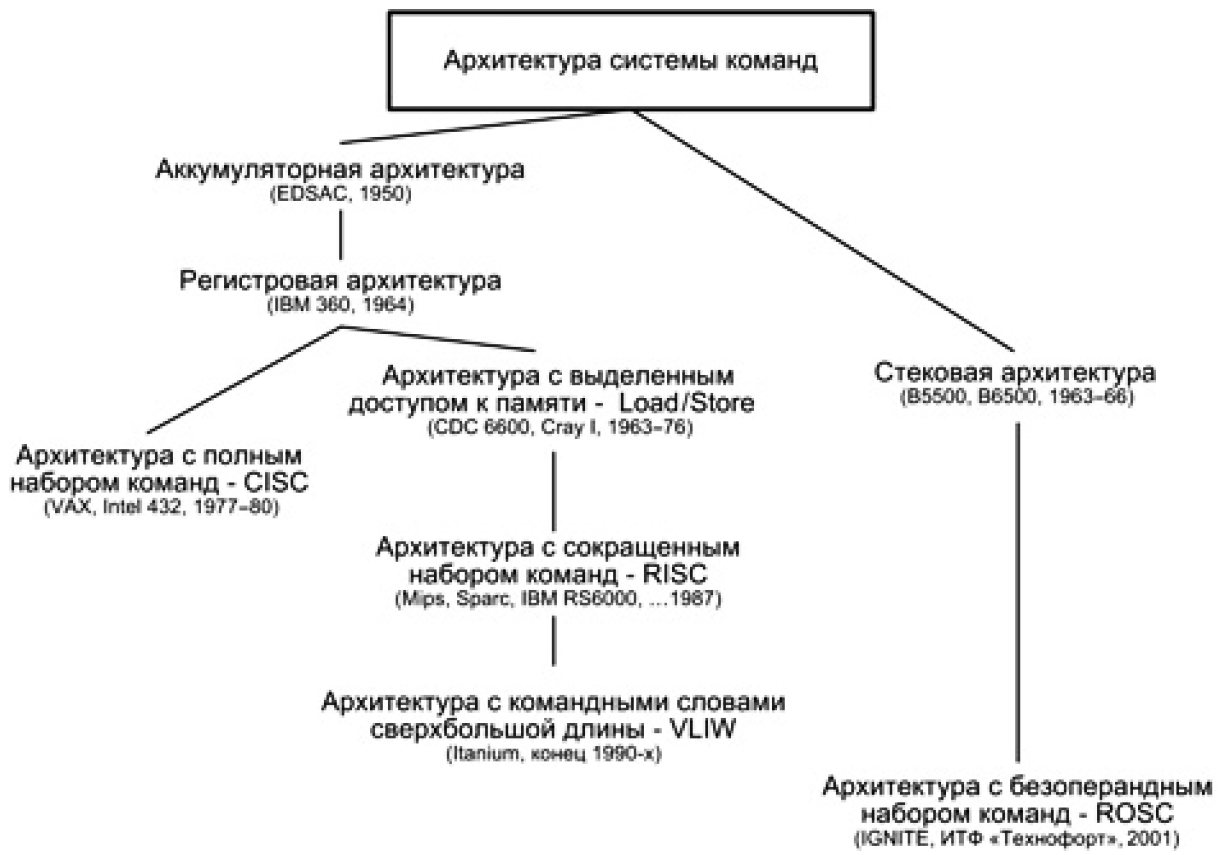
\includegraphics[width=0.7\textwidth]{img/11.instr_sets.png}
    \caption{Орлов С.А., Цилькер Б.Я. Организация ЭВМ и систем: Учебник для вузов. 2-е изд. — СПб.: Питер, 2011. — 688 с.}
    \end{figure}
\end{frame}

\begin{frame}{CISC}
    CISC — Complicated Instruction Set Computer

    \begin{outline}[itemize]
        \1 Много способов адресовать аргументы команд
        \1 Смешанная адресация — разные операнды из разных мест
        \1 Команды похожи на операторы языков высокого уровня
        \1 Ассемблер дружественный
        \1 Небольшое количество сильно умных команд
        \1 Реализованы при помощи микропрограмм
        \1 Машинный код экономный в смысле занимаемого места в памяти (многие «популярные» команды занимают 1 байт)
    \end{outline}

    Примеры:

    IBM/360..z-Architecture, Intel x86 и x86\_64, Intel 8080 и Zilog Z80
\end{frame}

\begin{frame}{RISC}
    RISC — Reduced Instruction Set Computer

    \begin{outline}[itemize]
        \1 Отдельные команды для обмена данными с памятью
        \1 Команды простые
            \2 Команды выполняются за фиксированное время (фиксированное количество тактов)
            \2 Это упрощает конвейеризацию
        \1 Некоторые «долгие» команды выполняются асинхронно
        \1 Ассемблер недружественный
            \2 Помните про «глупый всеядный» конвейер?
        \1 Машинный код не экономный, все команды занимают одно машинное слово
            \2 В некоторых режимах половину
    \end{outline}

    Примеры:

    Cray CDC 6600 (1960-е), и большинство новых семейств, начиная с 1980-х: MIPS, SPARC, ARM, RISC-V
\end{frame}

\begin{frame}{CISC vs RISC: недружественный ассемблер --- это страшно?}
        \alert{Нет.}
        \begin{figure}
            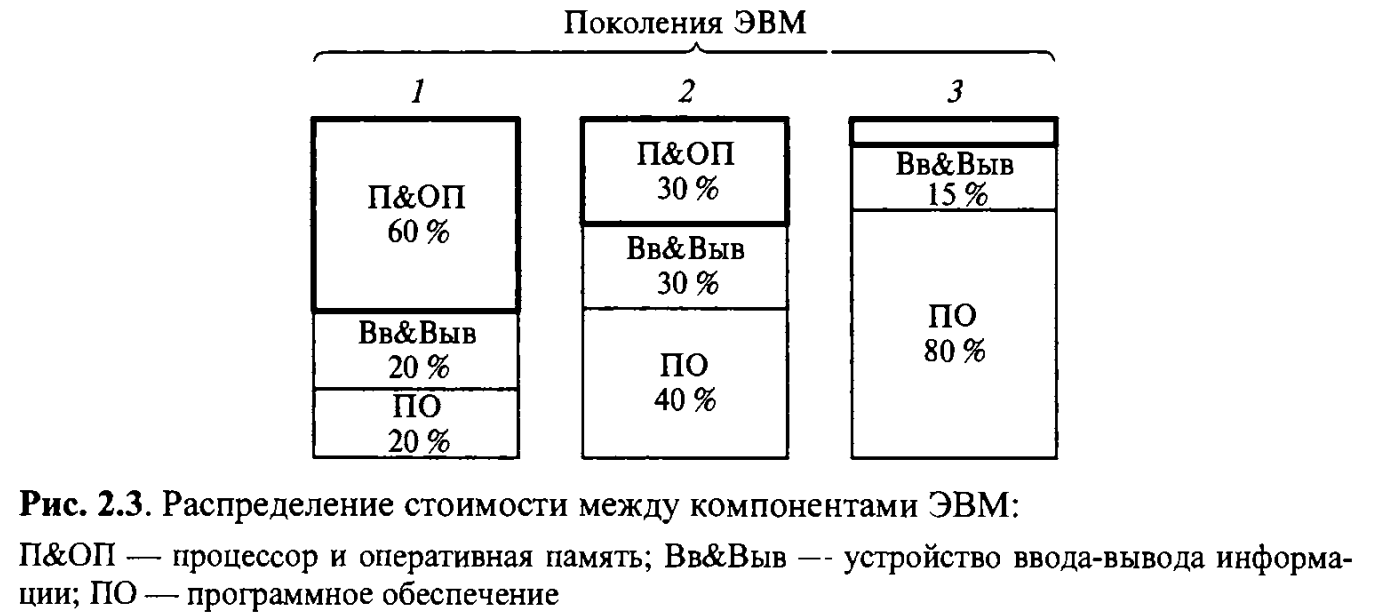
\includegraphics[width=0.8\textwidth]{img/11.generation_prices.png}
            \caption{Архитектура вычислительных систем.: Учеб. пособие. 2-e изд., перераб. и доп. M.: Изд-во МГТУ им. H.Э. Баумана, 2008. 520 c.}
        \end{figure}

        \begin{itemize}
            \item Cray CDC 6600 --- суперкомпьютер середины 1960-х, можно было программировать дорого, т.к. он и сам был очень дорогой
            \item Большинство --- 1980-е и позже, программируются уже на языках высокого уровня
        \end{itemize}
\end{frame}

\subsection{Особенности конвейеризации}

\begin{frame}{Конвейеризация в RISC}
    \begin{block}{Особенности и трудности}
        У RISC простой формат машинного кода, простой блок выборки инструкций, простой конвейер.
        Иногда есть несколько «долгих» команд, которые выполняются асинхронно
                \alert{Некоторые RISC-семейства не отслеживают конфликты и не обрабатывают их!}
    \end{block}

    \pause

    \begin{block}{Решения}
        \begin{itemize}
            \item Переупорядочивание команд — конфликтующие команды размещаются «на безопасном расстоянии» друг от друга
            \item Торможение при помощи вставки «пузырька» (инструкция nop, no operation)
        \end{itemize}
        \alert{Для некоторых RISC-семейств всё это делает компилятор или программист!}
    \end{block}
\end{frame}

\begin{frame}{Конвейеризация в CISC}
    Процессор полностью сам отвечает за корректное исполнение кода --- обнаруживает конфликты и обрабатывает их.

    ~

    Процессор с конвейером должен (кроме скорости) работать так же, как и без конвейера.
\end{frame}

\begin{frame}{Вопросы и упражнения}
\begin{block}{Вопросы}
\begin{itemize}
\tightlist
\item Назовите и определите основные блоки процессора.
\item Что такое вычислительный конвейер?
\item Во сколько раз может максимально ускорить выполнение программы конвейер, выполняющий команды в 3 этапа?
\item Назовите виды конфликтов конвейера.
\item Как RISC-процессоры разрешают конфликты конвейера?
\item Как CISC-процессоры разрешают конфликты конвейера?
\end{itemize}
\end{block}
\end{frame}

\postamble

\end{document}
